% !TeX spellcheck = de_AT_frami
\documentclass[10pt,a4paper]{article}
\usepackage[utf8x]{inputenc}
\usepackage{ucs}
\usepackage{amsmath,amsfonts,amssymb} % For math equations, theorems, sy
\usepackage{setspace}
\usepackage{amsfonts}
\usepackage{amssymb}
\usepackage{graphicx}
\usepackage{txfonts}
\usepackage[dvipsnames]{xcolor}
\usepackage{geometry}
\usepackage{graphicx}
\usepackage{epstopdf}
\epstopdfsetup{update}
\geometry{margin=2cm}
\usepackage[makeroom]{cancel}
\usepackage{multirow}
\setlength\parindent{0pt}

\usepackage{mdframed}
\usepackage{listings}

\usepackage{array}
\usepackage{mathtools} %for minus signs in matrices


\makeatletter
\def\zz\ignorespaces{\@ifnextchar-{}{\phantom{-}}}
\newcolumntype{R}{>{\zz}{r}}
\makeatother

\definecolor{mygreen}{RGB}{28,172,0} % color values Red, Green, Blue
\definecolor{mylilas}{RGB}{170,55,241}

\begin{document}
	\pagenumbering{gobble}

	\section*{9. Numerik Übungen 2017/18}
	\paragraph{T15}\mbox{}\\
	\textbf{%
		Es sei $\mathbf{R = [2,6]\times[1,3]}$ ein Rechteck. Berechnen Sie das Integral $\mathbf{\iint\limits_\text{R}\frac{x}{y}dF}$, indem Sie in x- bzw. y- Richtung die Simpsonregel verwenden. Machen Sie auch eine Skizze (Rechteck, Knoten, Gewichte).
	}\\\\
	Simpsonregel: $\qquad s=3, \qquad c=\left[ 0 \quad \frac{1}{2} \quad 1\right] , \qquad b=\left[ \frac{1}{6}\quad \frac{4}{6}\quad \frac{1}{6}\right] $ \\\\
	Quadraturformel für Rechtecke (4.103, S. 103):$ \qquad
		\iint\limits_\text{R}\frac{x}{y}\text{dF} \approx h\hat{h}\sum\limits_{i=1}^{s} \sum\limits_{j=1}^{\hat{s}}b_i\hat{b}_jf(a+c_ih,\,\hat{a}+\hat{c}_j\hat{h})$ \\
	Mit $h=b-a=6-2=4$ und $\hat{h}=\hat{b}-\hat{a}=3-1=2$  \\
	\begin{align*}
		h\hat{h}& = 4\cdot2 = 8
		\\\\
		b_i\hat{b}_j&=
		\begin{bmatrix}
			b_1\hat{b}_1 & b_1\hat{b}_2 & b_1\hat{b}_3 \\
			b_2\hat{b}_1 & b_2\hat{b}_2 & b_2\hat{b}_3 \\
			b_3\hat{b}_1 & b_3\hat{b}_2 & b_3\hat{b}_3
		\end{bmatrix}
		\overset{b_i=\hat{b}_j}{=}
		\begin{bmatrix}
			b_1b_1 & b_1b_2 & b_1b_3 \\
			b_2b_1 & b_2b_2 & b_2b_3 \\
			b_3b_1 & b_3b_2 & b_3b_3
		\end{bmatrix} = 
		\begin{bmatrix}
			\frac{1}{6}\cdot \frac{1}{6} & \frac{1}{6}\cdot \frac{4}{6} & \frac{1}{6}\cdot \frac{1}{6} \\
			\frac{4}{6}\cdot \frac{1}{6} & \frac{4}{6}\cdot \frac{4}{6} & \frac{4}{6}\cdot \frac{1}{6} \\
			\frac{1}{6}\cdot \frac{1}{6} & \frac{1}{6}\cdot \frac{4}{6} & \frac{1}{6}\cdot \frac{1}{6}
		\end{bmatrix} = 
		\frac{1}{36}\begin{bmatrix}
			1 & 4  & 1 \\
			4 & 16 & 4 \\
			1 & 4  & 1
		\end{bmatrix}
		\\\\
		f&\left( \begin{bmatrix}
			a+c_1h,\, \hat{a}+\hat{c}_1\hat{h} & a+c_1h,\, \hat{a}+\hat{c}_2\hat{h} & a+c_1h,\, \hat{a}+\hat{c}_3\hat{h} \\
			a+c_2h,\, \hat{a}+\hat{c}_1\hat{h} & a+c_2h,\, \hat{a}+\hat{c}_2\hat{h} & a+c_2h,\, \hat{a}+\hat{c}_3\hat{h} \\
			a+c_3h,\, \hat{a}+\hat{c}_1\hat{h} & a+c_3h,\, \hat{a}+\hat{c}_2\hat{h} & a+c_3h,\, \hat{a}+\hat{c}_3\hat{h}
		\end{bmatrix}\right) 
		=
		f\left( \begin{bmatrix}
			2+0\cdot 4,\, 1+0\cdot 2 & 2+0\cdot 4,\, 1+\frac{1}{2}\cdot 2 & 2+0\cdot 4,\, 1+1\cdot 2 \\
			2+\frac{1}{2}\cdot 4,\, 1+0\cdot 2 & 2+\frac{1}{2}\cdot 4,\, 1+\frac{1}{2}\cdot 2 & 2+\frac{1}{2}\cdot 4,\, 1+1\cdot 2 \\
			2+1\cdot 4,\, 1+0\cdot 2 & 2+1\cdot 4,\, 1+\frac{1}{2}\cdot 2 & 2+1\cdot 4,\, 1+1\cdot 2
		\end{bmatrix}\right)  = \\
		f&\left( \begin{bmatrix}
			2,\,1   & 2,\,2 & 2,\,3   \\
			4,\,1 & 4,\,2 & 4,\,3   \\
			6,\,1  & 6,\,2 & 6,\,3
		\end{bmatrix}\right) 
		=
		\begin{bmatrix}
			\frac{2}{1} & \frac{2}{2} & \frac{2}{3} \\
			\frac{4}{1} & \frac{4}{2} & \frac{4}{3} \\
			\frac{6}{1} & \frac{6}{2} & \frac{6}{3}
		\end{bmatrix}
		=
		\begin{bmatrix}
			2 & 1 & \frac{2}{3} \\
			4 & 2 & \frac{4}{3} \\
			6 & 3 & 2
		\end{bmatrix}
	\end{align*}
	\begin{align*}
		\iint\limits_\text{R}\frac{x}{y}\text{dF} &\approx 8\sum\limits_i\sum\limits_j
			\frac{1}{36}\begin{bmatrix}
				1 & 4  & 1 \\
				4 & 16 & 4 \\
				1 & 4  & 1
			\end{bmatrix}
			\begin{bmatrix}
				2 & 1 & \frac{2}{3} \\
				4 & 2 & \frac{4}{3} \\
				6 & 3 & 2
			\end{bmatrix}
			= \frac{8}{36}\sum\limits_i\sum\limits_j			
			\begin{bmatrix}
				2  & 4  & \frac{2}{3}  \\
				16 & 32 & \frac{16}{3} \\
				6  & 12 & 2
			\end{bmatrix} 
			=\frac{2}{9}\sum\limits_j\sum\limits_i
			2\begin{bmatrix}
				1 & 2  & \frac{1}{3} \\
				8 & 16 & \frac{8}{3} \\
				3 & 6  & 1
			\end{bmatrix}\\
			&=\frac{4}{9}\sum\limits_j
			\begin{bmatrix}
			    12 & 24 & 4
			\end{bmatrix} =
			\frac{4}{9}40 = \frac{160}{9}
	\end{align*}\\
	\begin{figure}[htbp]
		\centering
		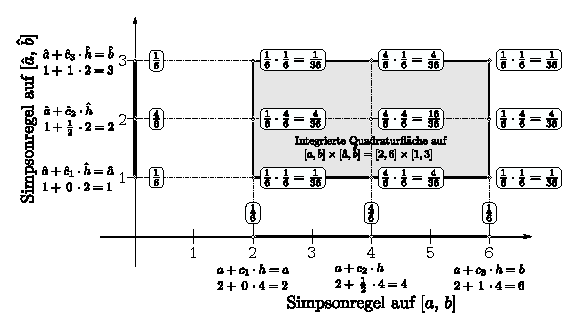
\includegraphics[width=0.8\textwidth]{T15.eps}
	\end{figure}
	\newpage
	\paragraph{T16}\mbox{}\\
	\textbf{%
	Die Knoten $\mathbf{(0,0), (1,0), (0,1)}$ und die Gewichte $\mathbf{\frac{1}{6},\frac{1}{6},\frac{1}{6}}$ definieren eine Quadraturformel auf dem Einheitsdreieck $\mathbf{D=\left\lbrace (\xi,\eta) \in \mathbb{R}^2 \,;\, 0\leq\xi\leq 1,\, 0\leq\eta \leq1-\xi \right\rbrace}$.\\
	Wie groß ist die Ordnung dieser Quadraturformel? \\
	Wie lauten die baryzentrischen Koordinaten der Knoten?
	} \\
	Nach 4.109 (S. 104) gilt
	\begin{align*}
		\sum_{i=1}^{s}b_ig(c_i,\,d_i)\approx\int\limits_{0}^{1}\int\limits_{0}^{1-\xi}g(\xi,\,\eta)\,\text{d}\eta\,\text{d}\xi.
	\end{align*}
	\begin{align*}
		\qquad s=3, \qquad \begin{pmatrix}c \\ d\end{pmatrix} 
		= \begin{pmatrix}0 \\ 0\end{pmatrix},\, 
		\begin{pmatrix}1 \\ 0\end{pmatrix}
		,\, \begin{pmatrix}0 \\ 1\end{pmatrix} , \qquad b=\left[ \frac{1}{6}\quad \frac{1}{6}\quad \frac{1}{6}\right] 
	\end{align*}
	Prüfen der Monome mit steigendem Grad \\
	\textbf{Grad 0:} 1
	\begin{align*}
		\int\limits_{0}^{1}\int\limits_{0}^{1-\xi}1\,\text{d}\eta\,\text{d}\xi =
		\int\limits_{0}^{1}1-\xi\,\text{d}\xi
	\end{align*}
	
	\newpage
	\paragraph{T17}\mbox{}\\
	\textbf{%
		a) Berechnen Sie die LU-Zerlegung der Matrix A mit Spaltenpivotsuche für
		\begin{align*}\mathbf{
			A= \begin{bmatrix}
				0   & 2   & 6  & 10 \\
				3   & 6   & 9  & -3 \\
				15  & 0   & 0  & 1  \\
				-15 & -10 & -3 & 1
			\end{bmatrix}.}
		\end{align*}
	}\\
    Analog zu \emph{5.1.2 Beispiel für eine LU-Zerlegung} führen wir einen Vektor \texttt{IP} von Seite 119 ein in dem wir Vertauschungen festhalten. Zu beginn tragen wir \texttt{IP}$(n=4)=(-1)^0=1$ ein.
    
    Wir suchen in der ersten Spalte nach dem Betragsmäßig größten Element von A. Dies trifft auf 15 und -15 zu, wobei hier 15 als Pivotelement gewählt wurde, da die dritten Zeile mehr Nullstellen enthält und wir uns somit Rechnungen sparen.
    
    Wir tauschen die 3. mit der 1. Zeile (\texttt{IP}$(1)=3$) und haben somit einmal getauscht (\texttt{IP}$(4)=(-1)^1=-1$).
    
    \begin{align*}
        \begin{tabular}{c|rrrr}
        	IP &     \multicolumn{4}{c}{\textbf{A}}     \\ \hline
        	*  &                      0 &   2 &  6 & 10 \\
        	*  &                      3 &   6 &  9 & -3 \\
        	*  & \colorbox{gray!20}{15}\hspace{-0.1cm} &   0 &  0 &  1 \\ \cline{1-1}
        	1  &                    -15 & -10 & -3 &  1
        \end{tabular}
	        \quad \rightarrow \quad
        \begin{tabular}{c|rrrr}
        	IP &                                       \multicolumn{4}{c}{\textbf{A}}                                       \\ \hline
        	3  & \colorbox{gray!20}{\textcolor{gray}{15}}\hspace{-0.1cm} & \textcolor{gray}{0} & \textcolor{gray}{0} & \textcolor{gray}{1} \\
        	*  &                                        3 &                   6 &                   9 &                  -3 \\
        	*  &                                        0 &                   2 &                   6 &                  10 \\ \cline{1-1}
        	-1 &                                      -15 &                 -10 &                  -3 &                   1
        \end{tabular}
    \end{align*}
    Die Faktoren für die Elimination sind
    \begin{align*}
	    l_{21} = \frac{a_{21}}{a_{11}} = \frac{3}{15} = \textcolor{Green}{\frac{1}{5}}, \qquad l_{31}=\frac{0}{15}=\textcolor{Fuchsia}{0}, \qquad l_{41}=\frac{-15}{15}=\textcolor{BrickRed}{-1}.
    \end{align*}
    Die Berechnung der Zeilenelemente erfolgt wie gewohnt. Die Nullstellen in der ersten Spalte werden jedoch mit den jeweiligen $l_{\text{j}1}$ ersetzt.
    
    Wir suchen im restlichen Bereich (schwarz) nach dem Pivotelement und finden -10. Getauscht wird die 4. mit der 2. Zeile.
    \begin{align*}
	    \begin{tabular}{c|rrrr}
	    	IP &                                   \multicolumn{4}{c}{\textbf{A}}                                   \\ \hline
	    	3  &             \textcolor{gray}{15} & \textcolor{gray}{0} & \textcolor{gray}{0} & \textcolor{gray}{1} \\
	    	*  & \textcolor{Green}{$\frac{1}{5}$} &                   6 &                   9 &     -$\frac{16}{5}$ \\
	    	*  &           \textcolor{Fuchsia}{0} &                   2 &                   6 &                  10 \\ \cline{1-1}
	    	-1 &         \textcolor{BrickRed}{-1} &                 \colorbox{gray!20}{-10}\hspace{-0.1cm} &                  -3 &                   2
	    \end{tabular}
		    \quad \rightarrow \quad
		\begin{tabular}{c|rrrr}
			IP &                                              \multicolumn{4}{c}{\textbf{A}}                                               \\ \hline
			3  &             \textcolor{gray}{15} &                       \textcolor{gray}{0} &  \textcolor{gray}{0} & \textcolor{gray}{1} \\
			4  &         \textcolor{BrickRed}{-1} & \colorbox{gray!20}{\textcolor{gray}{-10}}\hspace{-0.1cm} & \textcolor{gray}{-3} & \textcolor{gray}{2} \\
			*  &           \textcolor{Fuchsia}{0} &                                         2 &                    6 &                  10 \\ \cline{1-1}
			1  & \textcolor{Green}{$\frac{1}{5}$} &                                         6 &                    9 &     -$\frac{16}{5}$
		\end{tabular}
    \end{align*}
	\begin{align*}
		l_{32} = \frac{a_{32}}{a_{22}} = \frac{2}{-10} = \textcolor{Green}{-\frac{1}{5}}, \qquad l_{42}=\frac{6}{-10}=\textcolor{Fuchsia}{-\frac{3}{5}} \\
		\texttt{IP}(2)=4,\,\texttt{IP}(4)=(-1)^2=1\hspace{1.1cm}
	\end{align*}
	\begin{align*}
		\begin{tabular}{c|rrrr}
			IP &                                                     \multicolumn{4}{c}{\textbf{A}}                                                      \\ \hline
			3  &                   \textcolor{gray}{15} &                 \textcolor{gray}{0} &                \textcolor{gray}{0} & \textcolor{gray}{1} \\
			4  &            \textcolor{ProcessBlue}{-1} &               \textcolor{gray}{-10} &               \textcolor{gray}{-3} & \textcolor{gray}{2} \\
			*  &             \textcolor{ProcessBlue}{0} &   \textcolor{Green}{-$\frac{1}{5}$} &                     $\frac{27}{5}$ &      $\frac{52}{5}$ \\ \cline{1-1}
			1  & \textcolor{ProcessBlue}{$\frac{1}{5}$} & \textcolor{Fuchsia}{$-\frac{3}{5}$} & \colorbox{gray!20}{$\frac{36}{5}$}\hspace{-0.1cm} &                  -2
		\end{tabular}
			\quad \rightarrow \quad
		\begin{tabular}{c|rrrr}
			IP &                                                     \multicolumn{4}{c}{\textbf{A}}                                                      \\ \hline
			3  &                   \textcolor{gray}{15} &                 \textcolor{gray}{0} &                \textcolor{gray}{0} & \textcolor{gray}{1} \\
			4  &            \textcolor{ProcessBlue}{-1} &               \textcolor{gray}{-10} &               \textcolor{gray}{-3} & \textcolor{gray}{2} \\
			4  & \textcolor{ProcessBlue}{$\frac{1}{5}$} & \textcolor{Fuchsia}{$-\frac{3}{5}$} & \colorbox{gray!20}{$\frac{36}{5}$}\hspace{-0.1cm} & \textcolor{gray}{-2} \\ \cline{1-1}
			-1  &             \textcolor{ProcessBlue}{0} &   \textcolor{Green}{-$\frac{1}{5}$} &                     $\frac{27}{5}$ &      $\frac{52}{5}$
		\end{tabular}
	\end{align*}
	\begin{align*}
		l_{43} = \frac{a_{43}}{a_{33}} = \frac{\frac{27}{5}}{\frac{36}{5}} = \frac{27}{36} = \textcolor{Green}{\frac{3}{4}} \\
		\texttt{IP}(3)=4,\,\texttt{IP}(4)=(-1)^3=-1 \hspace{-0.3cm}
	\end{align*}
	\begin{align*}
		\begin{tabular}{c|rrrr}
			IP &                                                     \multicolumn{4}{c}{\textbf{A}}                                                      \\ \hline
			3  &                   \textcolor{gray}{15} &                 \textcolor{gray}{0} &                \textcolor{gray}{0} & \textcolor{gray}{1} \\
			4  &            \textcolor{ProcessBlue}{-1} &               \textcolor{gray}{-10} &               \textcolor{gray}{-3} & \textcolor{gray}{2} \\
			4  & \textcolor{ProcessBlue}{$\frac{1}{5}$} & \textcolor{ProcessBlue}{-$\frac{3}{5}$} & \textcolor{gray}{$\frac{36}{5}$}\hspace{-0.1cm} & \textcolor{gray}{-2} \\ \cline{1-1}
			-1  &             \textcolor{ProcessBlue}{0} &   \textcolor{ProcessBlue}{-$\frac{1}{5}$} &                     $\textcolor{Green}{\frac{3}{4}}$ &      $\frac{119}{10}$
		\end{tabular}
	\end{align*}
	\begin{align*}
		\text{L}=
		\begin{bmatrix}
			1                                    & 0                                     & 0                                    & 0 \\
			\textcolor{ProcessBlue}{-1}          & 1                                     & 0                                    & 0 \\
			\textcolor{ProcessBlue}{\frac{1}{5}} & \textcolor{ProcessBlue}{-\frac{3}{5}} & 1                                    & 0 \\
			\textcolor{ProcessBlue}{0}           & \textcolor{ProcessBlue}{-\frac{1}{5}} & \textcolor{ProcessBlue}{\frac{3}{4}} & 1
		\end{bmatrix}
			,\quad
		\text{U}=
		\begin{bmatrix}
			\textcolor{gray}{15} & \textcolor{gray}{0}   & \textcolor{gray}{0}                           & \textcolor{gray}{1}  \\
			0                    & \textcolor{gray}{-10} & \textcolor{gray}{-3}                          & \textcolor{gray}{2}  \\
			0                    & 0                     & \textcolor{gray}{\frac{36}{5}}\hspace{-0.1cm} & \textcolor{gray}{-2} \\
			0                    & 0                     & 0                                             & \textcolor{gray}{\frac{119}{10}}
		\end{bmatrix}
	\end{align*}



	\textbf{%
		b) Geben Sie auch die Permutationsmatrix P bzw. den Vektor \texttt{IP}. \texttt{IP(4)} soll das Vorzeichen für die Berechnung der Determinante erhalten.
	}\\
	Die Permutationsmatrix P ergibt sich durch Anwendung der Zeilentäusche auf eine Einheitsmatrix. Hierbei ist \texttt{IP} hilfreich.
	\begin{align*}
		\texttt{IP}=
		\begin{bmatrix}
			3 \\
			4 \\
			4 \\
			(-1)
		\end{bmatrix}
		, \quad
		\begin{bmatrix}
			1 & 0 & 0 & 0 \\
			0 & 1 & 0 & 0 \\
			0 & 0 & 1 & 0 \\
			0 & 0 & 0 & 1
		\end{bmatrix}
		\rightarrow
		\begin{bmatrix}
			0 & 0 & 1 & 0 \\
			1 & 0 & 0 & 0 \\
			0 & 1 & 0 & 0 \\
			0 & 0 & 0 & 1
		\end{bmatrix}
		\rightarrow
		\begin{bmatrix}
			0 & 0 & 1 & 0 \\
			0 & 0 & 0 & 1 \\
			0 & 1 & 0 & 0 \\
			1 & 0 & 0 & 0
		\end{bmatrix}
		\rightarrow
		\begin{bmatrix}
			0 & 0 & 1 & 0 \\
			0 & 0 & 0 & 1 \\
			1 & 0 & 0 & 0 \\
			0 & 1 & 0 & 0
		\end{bmatrix}
		= \text{P}
	\end{align*}
	\textbf{%
		c) Berechnen Sie mit Hilfe der LU-Zerlegung die Determinante von A.
	}\\
	Die Determinante kann mit U und $\texttt{IP}(n)$ berechnet werden.
	\begin{align*}\tag{5.38, S. 121}
		\det \text{A}& = u_{11}\cdot u_{22}\cdots u_{nn}\cdot\texttt{IP}(4) \\
		\det \text{A}& = 15\cdot -10 \cdot \frac{36}{5} \cdot \frac{119}{10} \cdot -1 =
			3\cdot  36 \cdot 119\\
			& = 12852
	\end{align*}
	
	\textbf{%
		d) Lösen Sie $\mathbf{Ax=b}$ für $\mathbf{b = \begin{bmatrix} 4 \\ -6 \\ -14  \\ -8 \end{bmatrix}}\,$ mit Hilfe der LU-Zerlegung.
	} \\
	Wiederum folgen wir dem Beispiel aus 5.1.2. \\
	\textbf{Schritt 1: Vertauschen der Elemente von b mit Hilfe von \texttt{IP}:}\\
	Wie in b) wenden wir IP auf b an.
	\begin{align*}
		\text{b} = \begin{bmatrix} 4 \\ -6 \\ -14  \\ -8 \end{bmatrix}
		\rightarrow
		\begin{bmatrix} -14 \\ -6 \\ 4  \\ -8 \end{bmatrix}
		\rightarrow
		\begin{bmatrix} -14 \\ -8 \\ 4  \\ -6 \end{bmatrix}
		\rightarrow
		\begin{bmatrix} -14 \\ -8 \\ -6  \\ 4 \end{bmatrix}
		= \tilde{\text{b}}
	\end{align*}
	\texttt{IP}$(4)=-1$ bedeutet eine ungerade Anzahl von Vertauschungen.\\
	\textbf{Schritt 2: Vorwärtssubstitution mit L und $\tilde{\text{b}}$:}
	\begin{figure}[htbp]
		\centering
		\begin{minipage}{0.4\linewidth}
			\begin{align*}
				\text{Ly}=
				\begin{bmatrix}
				1           & 0            & 0           & 0 \\
				-1          & 1            & 0           & 0 \\
				\frac{1}{5} & -\frac{3}{5} & 1           & 0 \\
				0           & -\frac{1}{5} & \frac{3}{4} & 1
				\end{bmatrix}
				\begin{bmatrix}
				y_1 \\
				y_2 \\
				y_3 \\
				y_4
				\end{bmatrix}
				= \begin{bmatrix} -14 \\ -8 \\ -6  \\ 4 \end{bmatrix}
				= \tilde{\text{b}}
			\end{align*}
		\end{minipage}
		\begin{minipage}{0.4\linewidth}
			\vspace{0.25cm}
			$\left\downarrow
			\begin{array}{rl}
				y_1=&\!\!\!\! -14 \\
				y_2=&\!\!\!\!  -8-(-14)\cdot -1 = -22 \\
				y_3=&\!\!\!\!  -6-(-14)\cdot \frac{1}{5}-(-22)\cdot-\frac{3}{5} = - \frac{82}{5}\\
				y_4=&\!\!\!\!  4-(-14)\cdot0-(-22)\cdot-\frac{1}{5}-(-\frac{82}{5})\cdot\frac{3}{4}   = \frac{119}{10}
			\end{array}
			\right.$
		\end{minipage}
	\end{figure}\\
	\textbf{Schritt 3: Rückwärtssubstitution mit U und y:}
	\begin{figure}[htbp]
		\centering
		\begin{minipage}{0.4\linewidth}
			\begin{align*}
			\text{Ux}=
			\begin{bmatrix}
				15 & 0   & 0            & 1              \\
				0  & -10 & -3           & 2              \\
				0  & 0   & \frac{36}{5} & -2             \\
				0  & 0   & 0            & \frac{119}{10}
			\end{bmatrix}
			\begin{bmatrix}
			x_1 \\
			x_2 \\
			x_3 \\
			x_4
			\end{bmatrix}
			= \begin{bmatrix} -14 \\ -22 \\ -\frac{82}{5}  \\ \frac{119}{10} \end{bmatrix}
			= \text{y}
			\end{align*}
		\end{minipage}
		\begin{minipage}{0.4\linewidth}
			\vspace{0.25cm}
			$\left\uparrow
			\begin{array}{rl}
			x_1=&\!\!\!\! \frac{1}{15}(-14-1) = -1 \\
			x_2=&\!\!\!\!  \frac{1}{-10} \left(-22-(-2)\cdot(-3)-1\cdot2 \right) = 3 \\
			x_3=&\!\!\!\! \frac{5}{36}\left( \frac{82}{5}-(1)\cdot(-2) \right) = -2\\
			x_4=&\!\!\!\! \frac{10}{119} \frac{119}{10} = 1
			\end{array}
			\right.$
		\end{minipage}
	\end{figure}
	\begin{align*}
		\text{x} = \begin{bmatrix}
		-1 \\
		3 \\
		-2 \\
		1
		\end{bmatrix}
	\end{align*}
	\newpage
	Matlab
	\lstset{language=Matlab,%
		%basicstyle=\color{red},
		breaklines=true,%
		morekeywords={matlab2tikz},
		keywordstyle=\color{blue},%
		morekeywords=[2]{1}, keywordstyle=[2]{\color{black}},
		identifierstyle=\color{black},%
		stringstyle=\color{mylilas},
		commentstyle=\color{mygreen},%
		showstringspaces=false,%without this there will be a symbol in the places where there is a space
		numbers=left,%
		numberstyle={\tiny \color{black}},% size of the numbers
		numbersep=9pt, % this defines how far the numbers are from the text
		emph=[1]{for,end,break},emphstyle=[1]\color{blue}, %some words to emphasise
		%emph=[2]{word1,word2}, emphstyle=[2]{style},    
	}
	\begin{mdframed}[linewidth=0pt,backgroundcolor=gray!10]
		\lstinputlisting{T17.m}
	\end{mdframed}
\end{document}
